\subsection{Kandidatensuche}
Die Kandidatensuche, im Folgenden Suche genannt, wird über eine klassische Graphensuche durchgeführt, wobei diese vom Ziel aus gestartet wird.
Der Root-Knoten definiert das zu treffende Ziel (Loch). Ein Knotenpunkt tieferer Ebene beinhaltet immer eine Kugel, welche
als nächst zu treffendes Ziel gilt. Eine Suche gilt als beendet, wenn die weisse Kugel als Knotenpunkt definiert wurde.
Der Expansionsschritt besteht darin, eine Kugel entweder direkt oder über die Bande anzuspielen,
wobei in dem Fall in diesem Schritt die gesamte Anzahl an anzuspielenden Banden abgetastet werden muss.
\\

Das Resultat der Expansion ist eine Abfolge von Knotenpunkten. Diese Knotenpunkte unterschieden sich von denen des
Suchbaums insofern, dass sie jeden Zusammenstoss abbilden. Das heisst, dass auch jeder Zusammenstoss mit der Bande
modelliert wird.
Am Ende der Expansion wird die minimal dem System zuzugebende Energie in Form des Geschwindigkeitsvektors der weissen
Kugel berechnet. Dazu wird das Resultat der Expansion vom Ziel aus abgearbeitet und nach jedem Knoten die Energie
berechnet, welche benötigt wird, um das Resultat zu erreichen.
\\

Um den Algorithmus vorzustellen, wird als Veranschaulichung ein Beispiel hinzugezogen. Es wird vereinfacht angenommen,
dass der Tisch nur ein Ziel hat. Für mehrere Ziele ergeben sich mehrere Suchbäume.
In Abbildung \ref{fig:backwardsearch_1} erfolgt die Eingabe des Suchalgorithmus in Form des Root-Knotens. Es wird nur das zu treffende Ziel
definiert. Auf der rechten Seite des Tisches wird einerseits der Suchbaum in Spalte 1 und andererseits das Resultat
des Algorithmus in Spalte 2 gezeigt. Das Resultat wird wiederum in Form von Ereignisknoten, wie in Kapitel \ref{kap:algorithmus_suche}
vorgestellt, angegeben.

\begin{figure}[h!]
    \begin{center}
        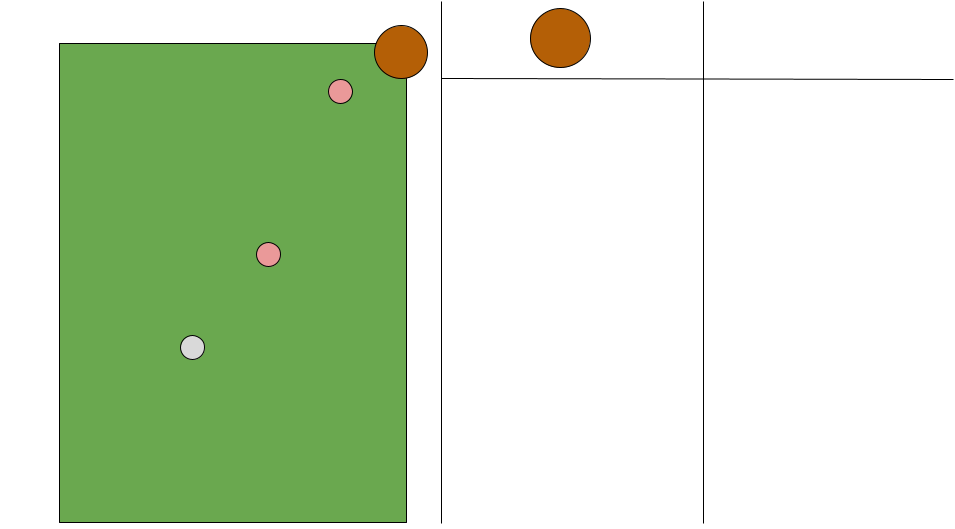
\includegraphics[width=0.5\linewidth]{../common/03_billiard_ai/resources/11_backwardsearch_1.png}
    \end{center}
    \caption{Kandidatensuche 1}
    \label{fig:backwardsearch_1}
\end{figure}

In einem zweiten Schritt wird die einzulochende Kugel definiert. Es kommen zwei Kugeln in Frage, wobei sich für eine
entschieden wird. Abbildung \ref{fig:backwardsearch_2} zeigt, dass der Suchbaum um einen Knoten erweitert wurde, das
Resultat definiert nun ebenso einen Endzustand. Dieser Endzustand bildet das Entfernen eines Objekts aus dem System aufgrund
der Kollision der Kugel mit dem Ziel ab.
\begin{figure}[h!]
    \begin{center}
        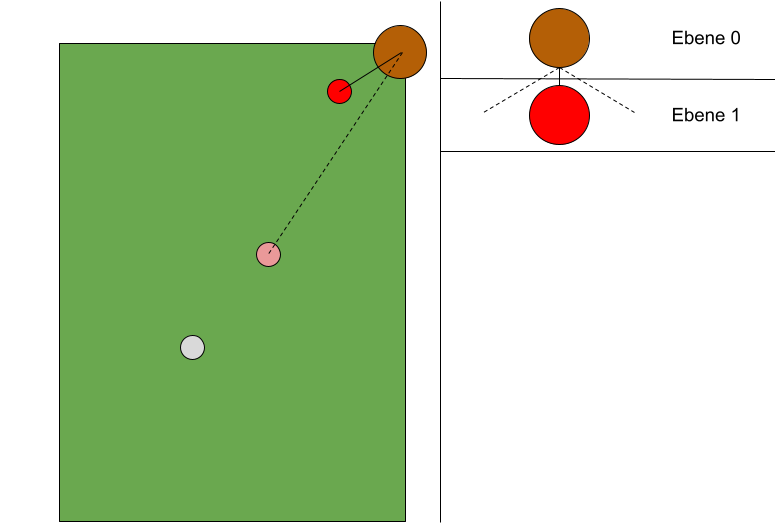
\includegraphics[width=0.5\linewidth]{../common/03_billiard_ai/resources/12_backwardsearch_2.png}
    \end{center}
    \caption{Kandidatensuche 2}
    \label{fig:backwardsearch_2}
\end{figure}

In Abbildung \ref{fig:backwardsearch_3} erfolgt der letzte Schritt. Auch hier ergeben sich diverse Optionen. Um den
Unterschied zwischen Suchbaum und Resultat aufzuzeigen, wird den Weg über eine Bande gewählt. Der Suchbaum beinhaltet
die weisse Kugel, die Suche gilt also als abgeschlossen. Das Resultat wiederum wird für jede Kollision um einen
Knoten erweitert. Am Ende wird noch ein \glqq Energy-Input-Node\grqq{} eingefügt.
\begin{figure}[h!]
    \begin{center}
        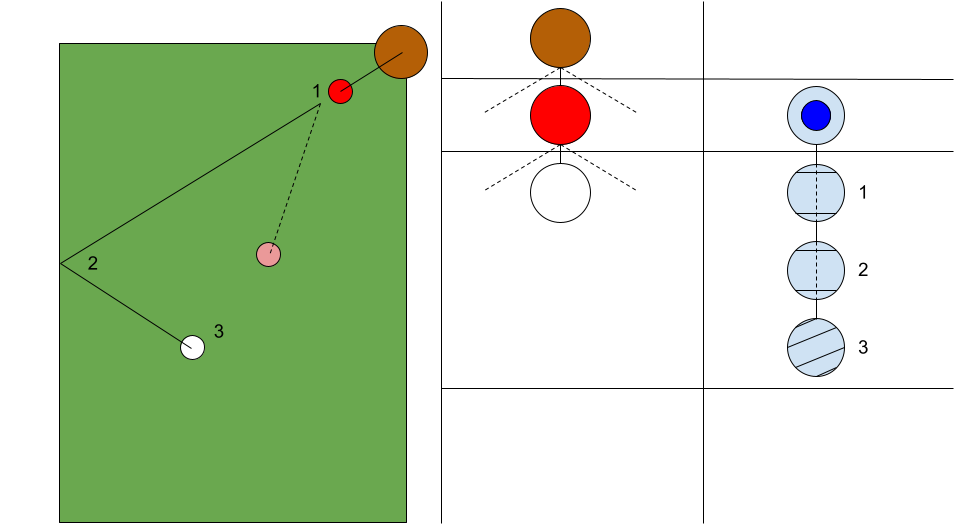
\includegraphics[width=0.5\linewidth]{../common/03_billiard_ai/resources/13_backwardsearch_3.png}
    \end{center}
    \caption{Kandidatensuche 3}
    \label{fig:backwardsearch_3}
\end{figure}

Resultatskette und Suchbaumpfad unterscheiden sich demnach markant, algorithmisch kann die Resultatskette den Pfad im Suchbaum aber
sehr gut nachbilden. So können in einem Expansionsschritt beliebig viele Kollisionsknoten eingefügt werden, wobei im
nächsten Expansionsschritt nur der letzte eingefügte Knoten relevant ist. Sollte die weisse Kugel expandiert werden,
wird zusätzlich noch ein \glqq Energy-Input-Node\grqq{} eingefügt und die Suche ist beendet.

\begin{algorithm}[H]
    \DontPrintSemicolon
    \SetKwFunction{expand}{expand}
    \SetKwProg{Fn}{Function}{}{}
    \Fn{\expand{node: Node, constantObjects: list} $\longrightarrow$ list[Node]}{
        nodes $\longleftarrow$ list()\\
        nodes $\longleftarrow$ append(expandBalls(node, constantObjects))\\
        nodes $\longleftarrow$ append(expandBank(node, constantObjects))\\
        \KwRet nodes
    }
    \caption{Algorithmus zur Durchführung eines Expansionsschritts bei der Kandidatensuche}
    \label{alg:backward_search}
\end{algorithm}

Anhand der Resultatskette wird abschliessend die Berechnung zur Eingabe der minimalen Energie durchgeführt.
Wie diese Energie berechnet wird, soll in den nächsten Abschnitten genauer erklärt werden.

\subsubsection{Reibungsverlust über Bahn}
TODO: T-5

\subsubsection{Energieübergabe bei Kugelkollision}
TODO: T-5
